\section{Formal grammars and syntactic parsing}
\begin{itemize}
	\item Syntax: structure of sentence, parsing syntax to get (long-distance) dependencies of words
\end{itemize}

\subsection{Generative grammar}
\begin{itemize}
	\item Formally specified grammar that can generate all and only acceptable sentences of a natural language
	\item A phrase can be bracketed into its internal structure: \textit{((the (big dog)) slept)}
	\item Each subpart is a \textbf{constituent}: group of words/phrase behaving as a single unit 
	\item Labels can be assigned to the internal structures (for instance, \textit{the big dog} is a noun phrase)
\end{itemize}
\subsubsection{Phrases and substitutability}
\begin{itemize}
	\item Words with the same POS tag can be replaced
	\item Phrasal categories indicate which phrases can be substituted
	\item Example phrasal categories include noun phrase (NP), verb phrase (VP), propositional phrase (PP), ...
	\item Goal: capture substitutability at phrase level by phrasal categories
\end{itemize}
\subsection{Context-Free Grammars}
\begin{itemize}
	\item Defining a grammar on rules of production, and basic lexicon
	\item Basic elements of a context-free grammar (CFG):
	\begin{enumerate}
		\item Set of non-terminal symbols (e.g. S, VP)
		\item Set of terminal symbols (i.e., the words)
		\item Set of rules, where left-hand side is single non-terminal symbol, and right side combination of non-terminal and terminal. Examples:\\
		\texttt{S -> NP VP}\\
		\texttt{V -> fish}
		\item A start symbol (here \texttt{S}) which is a non-terminal
	\end{enumerate}
	\item Exclude empty productions, like \texttt{NP->$\epsilon$}
	\item For rules of non-terminal to single word, the non-terminal represents the POS tag of this word
	\item A context free grammar can be used for either generating sentences (start with \texttt{S}, and choose rules), or for analyzing/assigning a structure to a given sentence
	\item For analyzing, the bracketed notation or a parse tree is often used to represent the structure:
	
	\texttt{(S (NP} \textit{they}\texttt{) (VP (V }\textit{fish}\texttt{)))}  (for parse tree, \texttt{S} would be root node and \texttt{NP} and \texttt{VP} its children a.s.o.)
	\item However, the grammar is not always unique 
	\begin{itemize}
		\item \textbf{Lexical ambiguity}: a word is more than once in the lexicon having different POS tag
		\item \textbf{Structural ambiguity}: multiple possible analysis because of multiple rules for same non-terminals
	\end{itemize}
\end{itemize}
\subsection{Chart parsing with CFGs}
\begin{itemize}
	\item Increase efficiency by recording all possible rules we could apply on a sentence
	\item The \textbf{chart} is a record of all substructures that have ever been built during the parsing / stores partial results of parsing in a vector
	\item An \textbf{edge} is a data structure that represents a rule application ,which includes:
	\begin{itemize}
		\item An id for referring to it
		\item The outer left and right node in the sentence of the phrase on which the rule is applied
		\item The \textit{mother} symbol (non-terminal which is on the left side of the rule)
		\item The \textit{daughters} which are the symbols on the right side of the rule (words and/or non-terminals produced by previous edges and referred to by the id)
	\end{itemize}
	\item In conclusion, a full chart for the sentence \texttt{they can fish} look like that:
%	$$\begin{array}{ccccc}
%	\text{id} & \text{left} & \text{right} & \text{mother} & \text{daugthers}\\
%	\hline
%	1 & 0 & 1 & \texttt{NP} & \text{(they)}\\
%	2 & 1 & 2 & \texttt{V} & \text{(can)}\\
%	3 & 1 & 2 & \texttt{VP} & \text{(2)}\\
%	4 & 0 & 2 & \texttt{S} & \text{(1 3)}\\
%	\end{array}$$
	$$\begin{array}{ccccc}
	\text{id} & \text{left} & \text{right} & \text{mother} & \text{daugthers}\\
	\hline
	1 & 0 & 1 & \texttt{NP} & \text{(they)}\\
	2 & 1 & 2 & \texttt{V} & \text{(can)}\\
	3 & 1 & 2 & \texttt{VP} & \text{(2)}\\
	4 & 0 & 2 & \texttt{S} & \text{(1 3)}\\
	5 & 2 & 3 & \texttt{V} & \text{(fish)}\\
	6 & 2 & 3 & \texttt{VP} & \text{(5)}\\
	7 & 1 & 3 & \texttt{VP} & \text{(2 6)}\\
	8 & 0 & 3 & \texttt{S} & \text{(1 7)}\\
	9 & 2 & 3 & \texttt{NP} & \text{(fish)}\\
	10 & 1 & 3 & \texttt{VP} & \text{(2 9)}\\
	11 & 0 & 3 & \texttt{S} & \text{(1 10)}\\
	\end{array}$$
	where the sentence is structured as $._0$\texttt{they}$._1$ \texttt{can}$._2$ \texttt{fish}$._3$ and rows of the chart are edges. The parsing is visualized in the figure below
	\begin{figure}[ht]
		\centering
		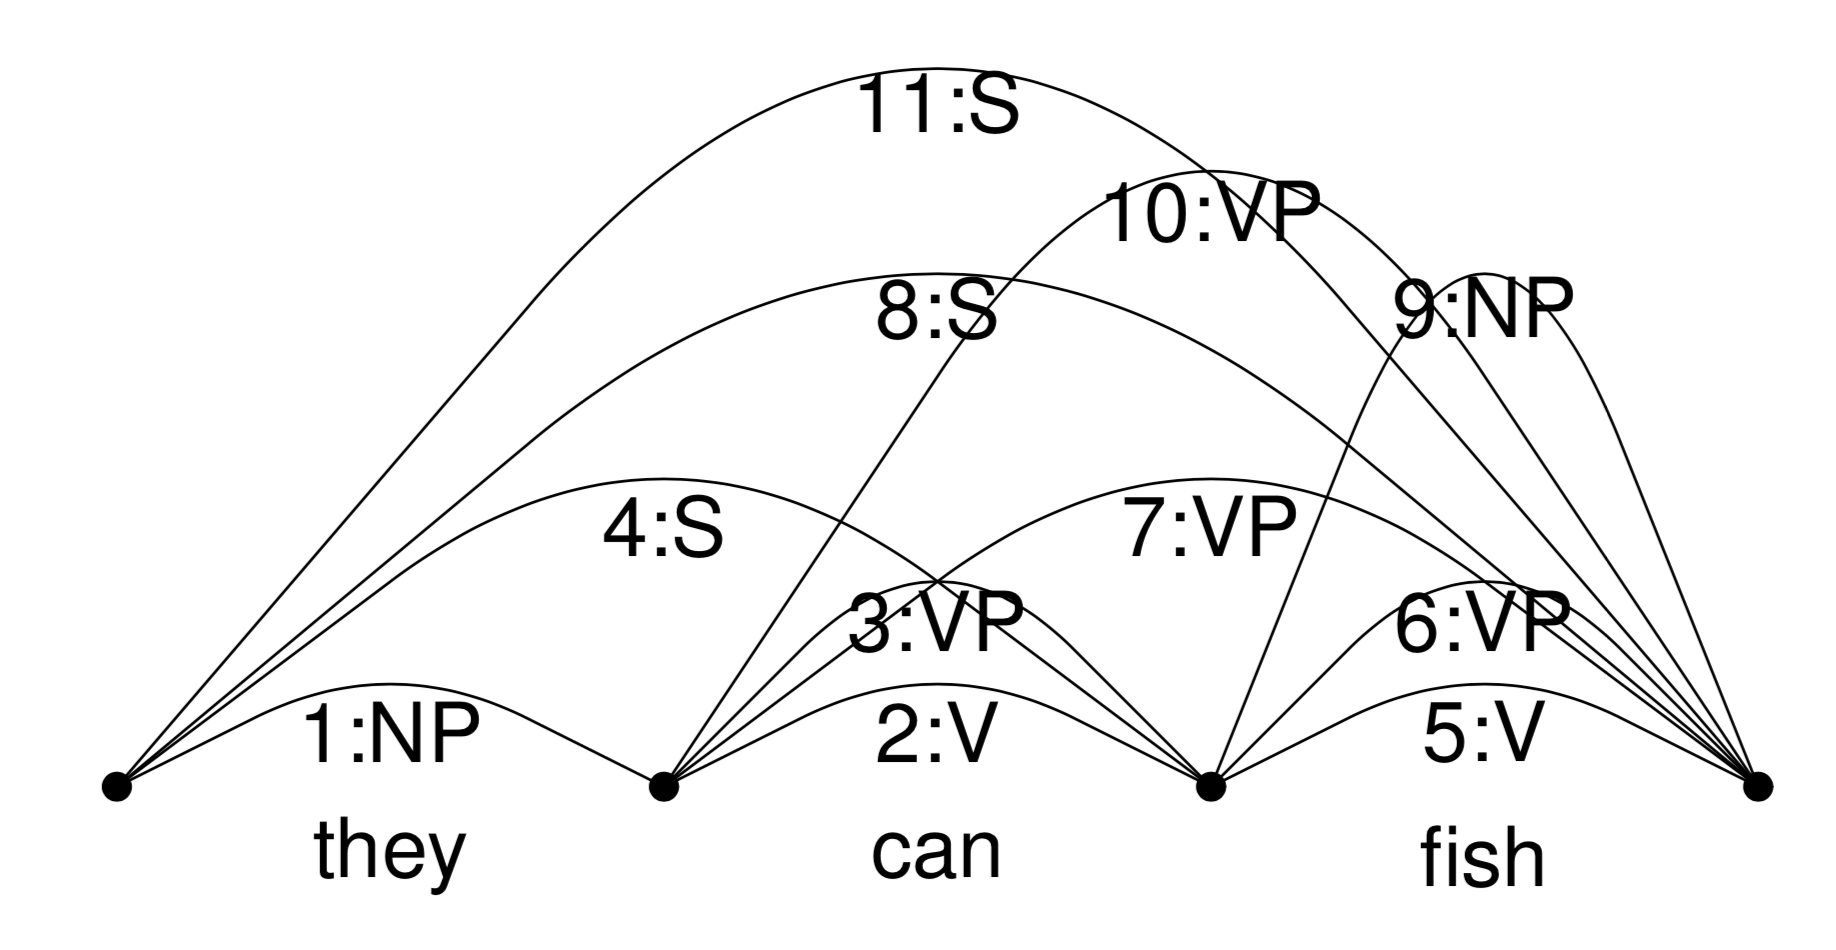
\includegraphics[width=0.5\textwidth]{figures/chart_parsing_structure.png}
		\caption{Example for chart parsing. The resulting chart data structure is shown below.}
		\label{fig:chart_parsing_structure}
	\end{figure}
\end{itemize}
\subsubsection{Implementation of bottom-up parser}
\begin{itemize}
	\item A bottom-up parser would start from the left, look at the first two connections points (first word) and check for a rule that can be applied to this word
	\item If a rule has been found, it is added as edge into the chart, and we start looking for rules that can be applied to the new edge (recursion!). Once no more rule can be applied on this edge and the recursion stops, we go back to the word and continue our search for applicable rules on this word 
	\item After every rule was applied, the parser moves on to the next word on the right and check for rules that can be applied to this word, \textbf{and} all other words/edges that have been processed beforehand. 
	\item Only if no more rules can be applied, the parser moves on to the next word, until all words are processed
	\item The correct parse/grammar structure is this one that end with the start symbol \texttt{S} from the first to the last node of the sentence
	\item Important sub-technique: \textbf{Packing}
	\begin{itemize}
		\item Due to multiple rules with same input, we can have two identical edges that are just based on different daughters
		\item Every following rule is then applied on both edges which is very inefficient
		\item Thus, with \textit{packing} we change the daughter entries to a list of possible daughter lists 
		\item For example, the edge 7 and 10 from the previous example can be combined:
		$$\begin{array}{ccccc}
		\text{id} & \text{left} & \text{right} & \text{mother} & \text{daugthers}\\
		\hline
		7 & 1 & 3 & \texttt{VP} & \left\{\text{(2 6), (2 9)}\right\}\\
		\end{array}$$
		\item If a new daughter list is added, no new recursion/rule application needs to be done  
	\end{itemize}
\end{itemize}
\subsection{Probabilistic parsing}
\begin{itemize}
	\item For a single sentence with 20 or more words, we will get over 1000 analysis $\Rightarrow$ how do we determine the best/most probable analysis?
	\item The traditional approach is it to grammar rules handwritten but they tend to often fail when parsing new sentences
	\item  Current approaches: probabilistic CFG (PCFG) where every rule is augmented with a probability
	\begin{figure}[ht]
		\centering
		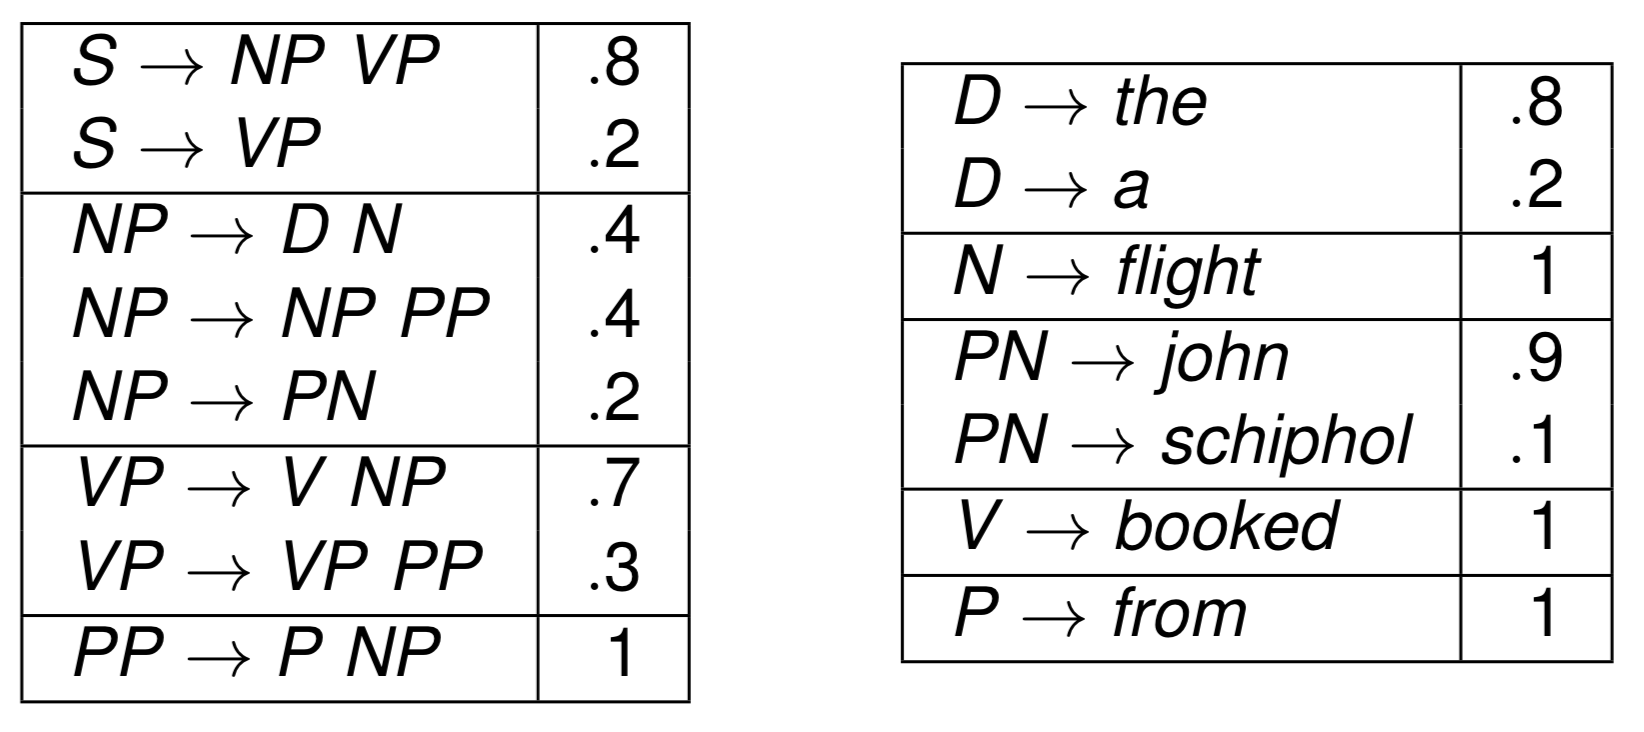
\includegraphics[width=0.35\textwidth]{figures/chart_parsing_prob_cfg.png}
		\caption{Probabilistic CFGs. The probabilities are normalized over all rules with same \textit{left} side.}
		\label{fig:probabilistic_cfg}
	\end{figure}
	\item The probability of a parse tree is the product of the probabilities of all the grammar rules that are used in the sentence derivation
	\item Probabilistic CFGs help for \textit{disambiguation} as we can rank all analysis by probability and just pick the best (n) one(s)
	\item Probabilities can also be used to speed up parsing (drop trees/substructures during parsing that already have a very low probability compared to other current substructures)
\end{itemize}
\subsubsection{Treebank PCFGs}
\begin{itemize}
	\item Instead of specifying/tuning the grammar and its corresponding probabilities by our own, we can use a large dataset of sentences with annotated parse trees
	\item This way, we implicitly get a grammar and the probabilities of each rule
	\item A \textbf{treebank} is therefore a collection of sentences annotated with constituent trees
	\item To estimate the rule probabilities, we use the maximum likelihood:
	$$p(X\to \alpha) = \frac{C(X\to \alpha )}{C(X)}$$
	where $C(X\to \alpha)$ number of times the rule is used in corpus, and $C(X)$ the number of times the non-terminal symbol $X$ appears in treebank
\end{itemize}
\subsubsection{Why CFG and not finite state machines}
\begin{itemize}
	\item Language often has centre-embeddings like $A\to \alpha A \beta$ which cannot be captures by FSAs
	\item However, humans limit the application of such centre-embeddings so that we can convert those into finite rules
	\item The advantage of a FSA would be that we can model hierarchical structures (supported by the fact that we understand the semantic of a sentence, we need good internal structures like the hierarchy)
\end{itemize}
\subsection{Dependency structures}
\begin{itemize}
	\item Context free grammars were based on phrase-structures in sentences
	\item Another possible representation of parsing sentences is using directed/asymmetric binary grammatical relations that hold among the words 
	\item A relation consists of 
	\begin{itemize}
		\item a head \texttt{H} (central word)
		\item a dependent \texttt{D}
		\item a label identifying the relation between \texttt{H} and \texttt{D}
	\end{itemize}
	\begin{figure}[ht]
		\centering
		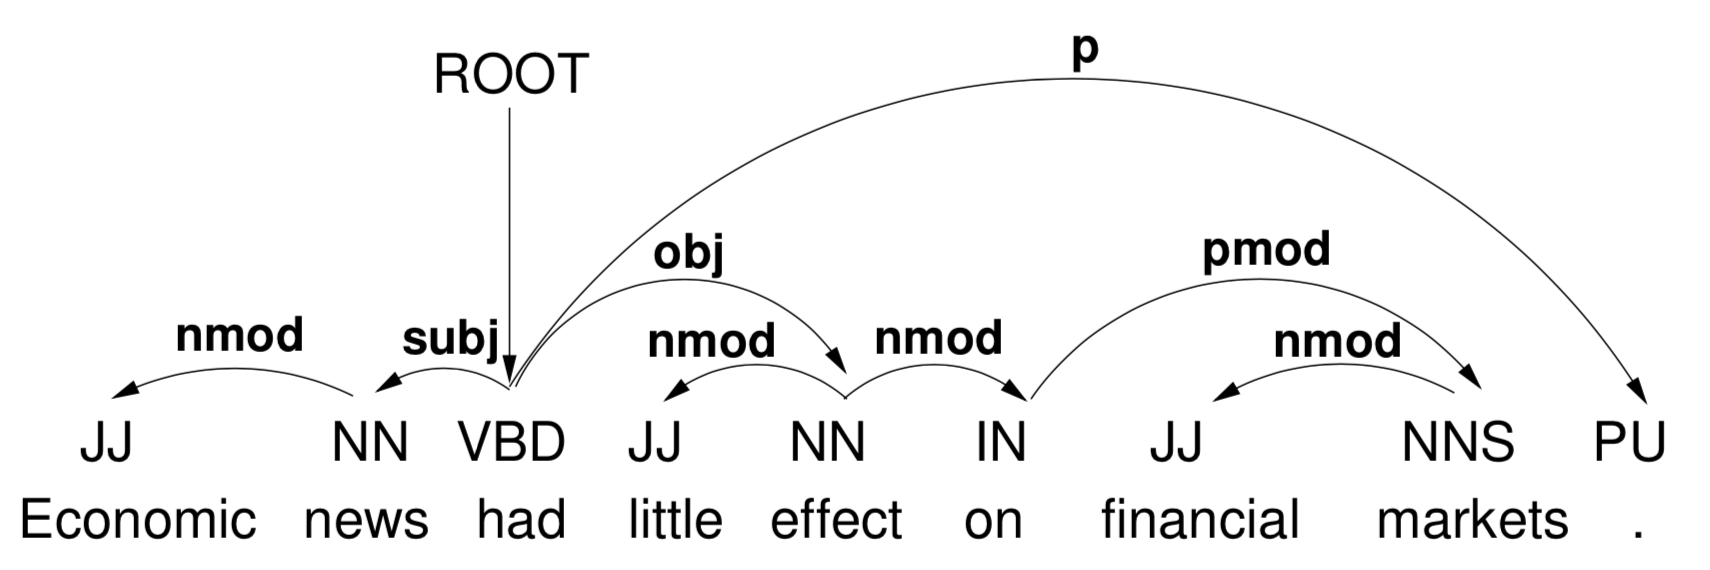
\includegraphics[width=0.5\textwidth]{figures/dependency_parsing.png}
		\caption{Dependency parsing. All relations are directed form head \texttt{H} to dependent \texttt{D}.}
		\label{fig:dependency_parsing}
	\end{figure}
	\item It is important to prevent parsing errors as these can significantly change the semantic of a sentence
\end{itemize}